%%%%%%%%%%%%%%%%%%%%%%%%%%%%%%%%%%%%%%%%%%%%%%%%%%%%%%%%%%%%%%%%%%%%%%%%%%%%%%%%%%
\begin{frame}[fragile]\frametitle{}
\begin{center}
{\Large K-Nearest Neighbors with Scikit-Learn}
\end{center}
\end{frame}


%%%%%%%%%%%%%%%%%%%%%%%%%%%%%%%%%%%%%%%%%%%%%%%%%%%%%%%%%%%%%%%%%%%%%%%%
\begin{frame}[fragile]\frametitle{K-Nearest Neighbors}
\begin{lstlisting}
# k-Nearest Neighbor
from sklearn import datasets
from sklearn import metrics
from sklearn.neighbors import KNeighborsClassifier
# load iris the datasets
dataset = datasets.load_iris()
# fit a k-nearest neighbor model to the data
model = KNeighborsClassifier()
model.fit(dataset.data, dataset.target)
print(model)
# make predictions
expected = dataset.target
predicted = model.predict(dataset.data)
# summarize the fit of the model
print(metrics.classification_report(expected, predicted))
print(metrics.confusion_matrix(expected, predicted))
\end{lstlisting}

{\tiny (Ref: Machine Learning Algorithm Recipes in scikit-learn - Jason Brownlee)}

\end{frame}

% %%%%%%%%%%%%%%%%%%%%%%%%%%%%%%%%%%%%%%%%%%%%%%%%%%%%%%%%%%%
% \begin{frame}[fragile]\frametitle{Knn Template Code}
% \begin{lstlisting}
% from sklearn.neighbors import KNeighborsClassifier 

% #Assumed you have, X (predictor) and Y (target) 
% # for training and x_test(predictor) of test 

% model = KNeighborsClassifier(n_neighbors=6)

% model.fit(X, y) 

% predicted= model.predict(x_test) 
% \end{lstlisting}
% \end{frame}

% %%%%%%%%%%%%%%%%%%%%%%%%%%%%%%%%%%%%%%%%%%%%%%%%%%%%%%%%%%%%%%%%%%%%%%%%%%%%%%%%%%
% \begin{frame}[fragile]\frametitle{}
% \begin{center}
% {\Large Test case: Iris Flowers}
% \end{center}
% \end{frame}



% %%%%%%%%%%%%%%%%%%%%%%%%%%%%%%%%%%%%%%%%%%%%%%%%%%%%%%%%%%%
% \begin{frame}[fragile]\frametitle{Review of the iris dataset}
% \begin{lstlisting}
% import pandas as pd

% url = 'http://archive.ics.uci.edu/ml/
		% machine-learning-databases/iris/iris.data'
		
% col_names = ['sepal_length', 'sepal_width', 'petal_length',
				% 'petal_width', 'species']
				
% iris = pd.read_csv(url, header=None, names=col_names)

% \end{lstlisting}
% \end{frame}

% %%%%%%%%%%%%%%%%%%%%%%%%%%%%%%%%%%%%%%%%%%%%%%%%%%%%%%%%%%%
% \begin{frame}[fragile]\frametitle{Review of the iris dataset}
% \begin{center}
% 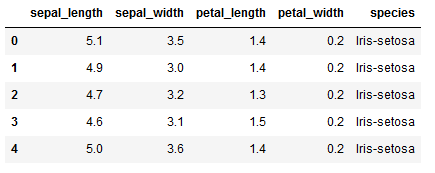
\includegraphics[width=0.8\linewidth,keepaspectratio]{knn8}
% \end{center}
% \begin{itemize}
% \item 150 observations (n=150): each observation is one iris flower
% \item 4 features: sepal length, sepal width, petal length, petal width
% \item Response: iris species
% \item Classification problem since response is categorical
% \end{itemize}
% \end{frame}


% %%%%%%%%%%%%%%%%%%%%%%%%%%%%%%%%%%%%%%%%%%%%%%%%%%%%%%%%%%%
% \begin{frame}[fragile]\frametitle{Encoding Iris dataset}
% Encoding of the Target
% \begin{lstlisting}
% iris['species_num'] = iris.species.map({'Iris-setosa':0, 
											% 'Iris-versicolor':1, 
											% 'Iris-virginica':2})
% \end{lstlisting}
% \end{frame}


% %%%%%%%%%%%%%%%%%%%%%%%%%%%%%%%%%%%%%%%%%%%%%%%%%%%%%%%%%%%
% \begin{frame}[fragile]\frametitle{Plot Iris dataset}
% Exploratory Data Analysis
% \begin{lstlisting}
% # create a scatter plot of PETAL LENGTH versus PETAL WIDTH 
% # and color by SPECIES
% iris.plot(kind='scatter', x='petal_length', y='petal_width', c='species_num', colormap=cmap_bold)

% # create a scatter plot of SEPAL LENGTH versus SEPAL WIDTH 
% # and color by SPECIES
% iris.plot(kind='scatter', x='sepal_length', y='sepal_width', c='species_num', colormap=cmap_bold)
% \end{lstlisting}
% \end{frame}

% %%%%%%%%%%%%%%%%%%%%%%%%%%%%%%%%%%%%%%%%%%%%%%%%%%%%%%%%%%%
% \begin{frame}[fragile]\frametitle{Plot Iris dataset}
% Exploratory Data Analysis
% \begin{center}
% 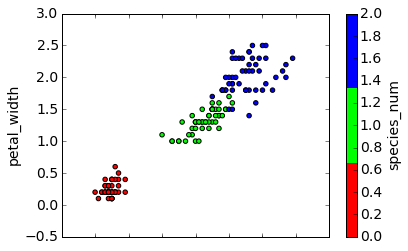
\includegraphics[width=0.4\linewidth,keepaspectratio]{knn9}

% 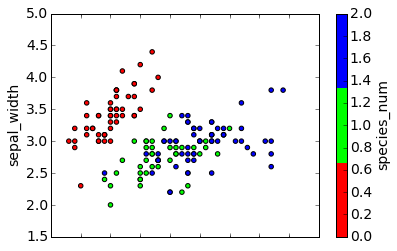
\includegraphics[width=0.4\linewidth,keepaspectratio]{knn10}
% \end{center}
% \begin{itemize}
% \item setosas have small petals, versicolor have medium sized petals and virginica have the largest petals. 
% \item Furthermore, setosas seem to have shorter and wider sepals than the other two classes. 
% \end{itemize}
% \end{frame}


% %%%%%%%%%%%%%%%%%%%%%%%%%%%%%%%%%%%%%%%%%%%%%%%%%%%%%%%%%%%
% \begin{frame}[fragile]\frametitle{KNN modeling}
% \begin{lstlisting}
% feature_cols = ['sepal_length', 'sepal_width', 
				% 'petal_length', 'petal_width']
				
% X = iris[feature_cols]
% y = iris.species_num

% from sklearn.neighbors import KNeighborsClassifier

% knn = KNeighborsClassifier(n_neighbors=1)

% knn.fit(X, y)

% knn.predict([3, 5, 4, 2]) # 2

% X_new = [[3, 5, 4, 2], [5, 4, 3, 2]]
% knn.predict(X_new) # 2,1
% \end{lstlisting}
% \end{frame}



% %%%%%%%%%%%%%%%%%%%%%%%%%%%%%%%%%%%%%%%%%%%%%%%%%%%%%%%%%%%
% \begin{frame}[fragile]\frametitle{Measuring Error}
% With $k=1$
% \begin{lstlisting}
% from sklearn.cross_validation import train_test_split

% X_train, X_test, Y_train, Y_test = train_test_split(
				% X,y, test_size=0.4, random_state=4)
				
% actual = Y_test

% knn = KNeighborsClassifier(n_neighbors=1)
% knn.fit(X_train, Y_train)
% expected = knn.predict(X_test) #predictions

% import sklearn.metrics
% score_1 = metrics.accuracy_score(actual, expected)
% print(score_1) #0.94

% \end{lstlisting}
% \end{frame}

% %%%%%%%%%%%%%%%%%%%%%%%%%%%%%%%%%%%%%%%%%%%%%%%%%%%%%%%%%%%
% \begin{frame}[fragile]\frametitle{Measuring Error}
% Try range of k values
% \begin{lstlisting}
% import matplotlib.pyplot as plt
    
% scores = []
% k_range = range(1,26)
% for k in k_range:
    % knn=KNeighborsClassifier(n_neighbors=k)
    % knn.fit(X_train, Y_train)
    % actual = knn.predict(X_test)
    % scores.append(metrics.accuracy_score(Y_test, actual))

% plt.xlabel('Value of K for KNN')
% plt.ylabel('Testing Accuracy')
% plt.plot(k_range, scores)
% plt.show()
% \end{lstlisting}
% \end{frame}


% %%%%%%%%%%%%%%%%%%%%%%%%%%%%%%%%%%%%%%%%%%%%%%%%%%%%%%%%%%%
% \begin{frame}[fragile]\frametitle{Effect of K}
% K=1,5, 15,50
% \begin{center}
% 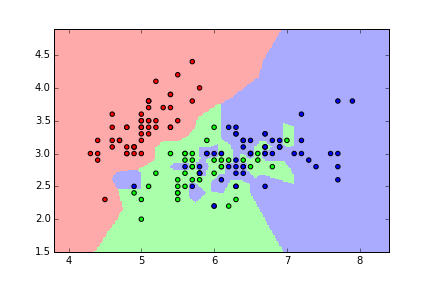
\includegraphics[width=0.4\linewidth,keepaspectratio]{knn11}
% 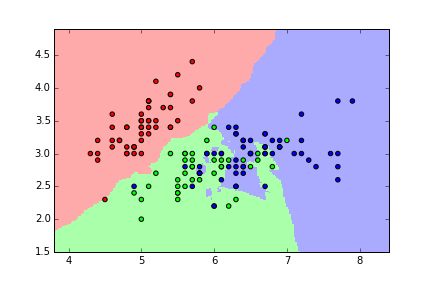
\includegraphics[width=0.4\linewidth,keepaspectratio]{knn12}\\
% 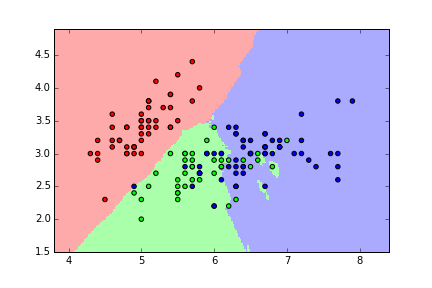
\includegraphics[width=0.4\linewidth,keepaspectratio]{knn13}
% 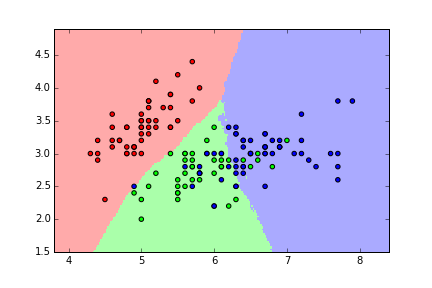
\includegraphics[width=0.4\linewidth,keepaspectratio]{knn14}
% \end{center}
% %Question: What's the ``best'' value for K in this case?\\
% %Answer: The one giving accurate predictions on unseen data.
% \end{frame}

% %%%%%%%%%%%%%%%%%%%%%%%%%%%%%%%%%%%%%%%%%%%%%%%%%%%%%%%%%%%%%%%%%%%%%%%%%%%%%%%%%%
% \begin{frame}[fragile]\frametitle{}
% \begin{center}
% {\Large Test case: NBA Players}
% \end{center}
% \end{frame}

% %%%%%%%%%%%%%%%%%%%%%%%%%%%%%%%%%%%%%%%%%%%%%%%%%%%%%%%%%%%
% \begin{frame}[fragile]\frametitle{Exercise}
% A look at the data, Each row in the data contains information on how a player performed in the 2013-2014 NBA season.
% \begin{lstlisting}
% import pandas
% with open("nba_2013.csv", 'r') as csvfile:
    % nba = pandas.read_csv(csvfile)

% # The names of all the columns in the data.
% print(nba.columns.values)
% \end{lstlisting}
% \end{frame}

% %%%%%%%%%%%%%%%%%%%%%%%%%%%%%%%%%%%%%%%%%%%%%%%%%%%%%%%%%%%
% \begin{frame}[fragile]\frametitle{Exercise}
% Here are some selected columns from the data:
% \begin{itemize}
% \item     player - name of the player
% \item     pos - the position of the player
% \item     g - number of games the player was in
% \item     gs - number of games the player started
% \item     pts - total points the player scored
% \end{itemize}
% There are many more columns in the data, mostly containing information about average player game performance over the course of the season.
% \end{frame}

% %%%%%%%%%%%%%%%%%%%%%%%%%%%%%%%%%%%%%%%%%%%%%%%%%%%%%%%%%%%
% \begin{frame}[fragile]\frametitle{Exercise}
% Study distance: find the most similar NBA players to Lebron James.
% \begin{lstlisting}
% selected_player = nba[nba["player"] == "LeBron James"].iloc[0]

% distance_columns = ['age', 'g', 'gs', 'mp', 'fg', 'fga', 
						% 'fg.', 'x3p', 'x3pa', 'x3p.', 'x2p',
						 % 'x2pa', 'x2p.', 'efg.', 'ft', 'fta',
						  % 'ft.', 'orb', 'drb', 'trb', 'ast', 'stl', 
						  % 'blk', 'tov', 'pf', 'pts']

% def euclidean_distance(row):
    % inner_value = 0
    % for k in distance_columns:
        % inner_value += (row[k] - selected_player[k]) ** 2
    % return math.sqrt(inner_value)


% lebron_distance = nba.apply(euclidean_distance, axis=1)
% \end{lstlisting}
% \end{frame}

% %%%%%%%%%%%%%%%%%%%%%%%%%%%%%%%%%%%%%%%%%%%%%%%%%%%%%%%%%%%
% \begin{frame}[fragile]\frametitle{Exercise}
% Normalizing columns
% \begin{lstlisting}
% # Select only the numeric columns from the NBA dataset
% nba_numeric = nba[distance_columns]

% # Normalize all of the numeric columns
% nba_normalized = (nba_numeric - nba_numeric.mean()) / nba_numeric.std()


% # Fill in NA values in nba_normalized
% nba_normalized.fillna(0, inplace=True)
% \end{lstlisting}
% \end{frame}

% %%%%%%%%%%%%%%%%%%%%%%%%%%%%%%%%%%%%%%%%%%%%%%%%%%%%%%%%%%%
% \begin{frame}[fragile]\frametitle{Exercise}
% Use the distance.euclidean function from scipy.spatial, a much faster way to calculate euclidean distance.
% \begin{lstlisting}
% # Find the normalized vector for lebron james.
% lebron_normalized = nba_normalized[nba["player"] == "LeBron James"]

% # Find the distance between lebron james and everyone else.
% euclidean_distances = nba_normalized.apply(lambda row: distance.euclidean(row, lebron_normalized), axis=1)

% # Create a new dataframe with distances.
% distance_frame = pandas.DataFrame(data={"dist": euclidean_distances, "idx": euclidean_distances.index})
% distance_frame.sort("dist", inplace=True)
% # Find the most similar player to lebron (the lowest distance to lebron is lebron, the second smallest is the most similar non-lebron player)
% second_smallest = distance_frame.iloc[1]["idx"]
% most_similar_to_lebron = nba.loc[int(second_smallest)]["player"]
% \end{lstlisting}
% \end{frame}

% %%%%%%%%%%%%%%%%%%%%%%%%%%%%%%%%%%%%%%%%%%%%%%%%%%%%%%%%%%%
% \begin{frame}[fragile]\frametitle{Exercise}
% Generating training and testing sets
% \begin{lstlisting}
% import random
% from numpy.random import permutation

% # Randomly shuffle the index of nba.
% random_indices = permutation(nba.index)

% # Set a cutoff for how many items we want in the test set (in this case 1/3 of the items)
% test_cutoff = math.floor(len(nba)/3)

% # Generate the test set by taking the first 1/3 of the randomly shuffled indices.
% test = nba.loc[random_indices[1:test_cutoff]]

% # Generate the train set with the rest of the data.
% train = nba.loc[random_indices[test_cutoff:]]
% \end{lstlisting}
% \end{frame}

% %%%%%%%%%%%%%%%%%%%%%%%%%%%%%%%%%%%%%%%%%%%%%%%%%%%%%%%%%%%
% \begin{frame}[fragile]\frametitle{Exercise}
% Using sklearn for k nearest neighbors
% \begin{lstlisting}
% x_columns = ['age', 'g', 'gs', 'mp', 'fg', 'fga', 'fg.', 'x3p', 'x3pa', 'x3p.', 'x2p', 'x2pa', 'x2p.', 'efg.', 'ft', 'fta', 'ft.', 'orb', 'drb', 'trb', 'ast', 'stl', 'blk', 'tov', 'pf']

% y_column = ["pts"]

% from sklearn.neighbors import KNeighborsRegressor

% knn = KNeighborsRegressor(n_neighbors=5)

% knn.fit(train[x_columns], train[y_column])

% predictions = knn.predict(test[x_columns])
% \end{lstlisting}
% \end{frame}

% %%%%%%%%%%%%%%%%%%%%%%%%%%%%%%%%%%%%%%%%%%%%%%%%%%%%%%%%%%%
% \begin{frame}[fragile]\frametitle{Exercise}
% Computing error
% \begin{lstlisting}
% actual = test[y_column]

% mse = (((predictions - actual) ** 2).sum()) / len(predictions)
% \end{lstlisting}
% \end{frame}

% %%%%%%%%%%%%%%%%%%%%%%%%%%%%%%%%%%%%%%%%%%%%%%%%%%%
% \begin{frame}[fragile] \frametitle{Classifier Comparison}

% \adjustbox{valign=t}{
% \begin{minipage}{0.45\linewidth}
% Eager Learners
% \begin{itemize}
% \item Decision Trees, SVMs
% \item Model Building: potentially slow 
% \item Classifying Test Instance: fast
% \item finding a global model that fits the entire input space

% \end{itemize}

% \end{minipage}
% }
% \hfill
% \adjustbox{valign=t}{
% \begin{minipage}{0.45\linewidth}
% Lazy Learners
% \begin{itemize}
% \item Nearest Neighbors
% \item Model Building: fast (because there is none!)
% \item Classifying Test Instance: slow
% \item classification decisions are made locally (small k values), and are more susceptible to noise
% \end{itemize}

% \end{minipage}
% }
% \end{frame}
